%! suppress = EscapeHashOutsideCommand
%! Author = Theodore Capinski
%! Date = 3/5/2024

% Preamble
\documentclass[11pt]{article}
\let\oldsection\section
\renewcommand\section{\clearpage\oldsection}
\setcounter{section}{-1}
\counterwithin{figure}{section}

% Packages
\usepackage{amsmath}
\usepackage{hyperref}
\usepackage{graphicx}
\usepackage{tikz}
\usepackage{indentfirst}
\usepackage{circuitikz}
\usepackage{calc}

%%%%%%%%%%%%%%%%%%%%%%%%%%%%%%%%%%%%%%%%%%%%%%%%%%%%%%%%%%%%%%%%%%%%%%
% LaTeX Overlay Generator - Annotated Figures v0.0.1
% Created with http://ff.cx/latex-overlay-generator/
%%%%%%%%%%%%%%%%%%%%%%%%%%%%%%%%%%%%%%%%%%%%%%%%%%%%%%%%%%%%%%%%%%%%%%
%\annotatedFigureBoxCustom{bottom-left}{top-right}{label}{label-position}{box-color}{label-color}{border-color}{text-color}
\newcommand*\annotatedFigureBoxCustom[8]{\draw[#5,thick,rounded corners] (#1) rectangle (#2);\node at (#4) [fill=#6,thick,shape=circle,draw=#7,inner sep=2pt,font=\sffamily,text=#8] {\textbf{#3}};}
%\annotatedFigureBox{bottom-left}{top-right}{label}{label-position}
\newcommand*\annotatedFigureBox[4]{\annotatedFigureBoxCustom{#1}{#2}{#3}{#4}{white}{white}{black}{black}}
\newcommand*\annotatedFigureText[4]{\node[draw=none, anchor=south west, text=#2, inner sep=0, text width=#3\linewidth,font=\sffamily] at (#1){#4};}
\newenvironment {annotatedFigure}[1]{\centering\begin{tikzpicture}
                                                   \node[anchor=south west,inner sep=0] (image) at (0,0) { #1};\begin{scope}[x={(image.south east)},y={(image.north west)}]}{\end{scope}\end{tikzpicture}}
%%%%%%%%%%%%%%%%%%%%%%%%%%%%%%%%%%%%%%%%%%%%%%%%%%%%%%%%%%%%%%%%%%%%%%

\newcommand{\todo}[1]{\textcolor{red}{TODO: #1}\PackageWarning{TODO:}{#1!}}

\title{Physics 5BL Lab Report EM1}
\author{T.~Capinski \and A.~Patel}

% Document
\begin{document}
    \maketitle
    \tableofcontents

    \section*{Introduction}\label{sec:introduction}
    \addcontentsline{toc}{section}{Introduction}

    This report will cover the Ohm's Law lab.
    We will be employing tools such as the Digital Multimeter (DMM) and the IOLab apparatus.
    Through measurements of resistance, current, and voltage, we will measure Ohmic and non-Ohmic behaviors in circuit elements, distinguishing between components that adhere to Ohm's Law and those that exhibit nonlinear characteristics.

    In addition, the lab will incorporate the application of Kirchhoff's Circuit Rules, which are used for analyzing circuit configurations.
    By employing the Junction Rule and Loop Rule, we can gain insight into the conservation of charge and energy within electrical circuits.

    For experiment 0, we simply measured the resistance of a 1 $\Omega$ resistor, however, we found that our measurement was outside the expected range of values using .01 $\Omega$ as the error in the resistors measurement. 

    For experiment 1A, we first measured the transfer ratio $(H \equiv V_{out} /V_{in})$ of a circuit with two 1000 $\Omega$ resistors in it, which we found to be .5005, inside the range of error for the accepted value of 0.5. we then used the DMM to measure voltage, comparing this to our voltage from the previous part, and finding that they both agreed with each other.
    For experiment 1B, we created a circuit with a 10,000 $\Omega$ resistor in it and measured the current using both the IOLab and the DMM. Our measured current from the IOLab was 0.229 mA, slightly out of the range of the accepted value of 0.2 mA. However, when using the DMM, we measured exactly 0.2 mA. We then determined the IOLab had higher sensitivity due to the large number of decimals it gave and its high error from the expected value.

    For experiment 2A, we first measured the current across a 10,000 $\Omega$ resistor to measure ohmic behavior.
    We used 10 different input voltages and found that it obeyed Ohm's law.
    We then calculated the resistance of the resistor to be $9379.79 \pm 233.97 \Omega$, which is slightly out of range of the accepted value.
    For experiment 2B, we measured the voltage across two LEDs to test for ohmic behavior.
    We used a 1000 $\Omega$ resistor in series to limit current and again took 10 data points for each LED\@.
    We found that both green and red LEDs did not obey Ohm's law, as they both needed a minimum voltage difference to let current through, then acted like wires.
    We also found the resistance of the resistor to be $996.50 \pm 2.56 \Omega$ when using the green LED and $989.35 \pm 10.81 \Omega$ when using the red LED, which were both inside the acceptable range of values.
    This is because the LED acted like a wire once the minimum voltage was met, so it allowed us to properly measure resistance.

    For experiment 3, we measured the current across different resistors in a circuit involving multiple batteries and resistors.
    Our data did not match the predicted values, and we could not verify Kirchhoff's junction rule equation.
    
    \section*{Theory}\label{sec:theory}
    Ohm's law states that the current through a conductor between two points is directly proportional to the voltage across the two points.
    This relationship is represented by the equation
    \begin{equation}\label{eq:ohm_equation}
        V = I \cdot R
    \end{equation}
    where $V$ is the voltage, $I$ is the current, and $R$ is the resistance.
    Such a relationship is linear and is known as ohmic behavior.
    To find the resistance of a material, we can use the equation
    \begin{equation}\label{eq:resistance_equation}
        R = \frac{V}{I}
    \end{equation}

    As covered in the report overview, resistors in series can be summed up, such as
    \begin{equation}\label{eq:resistors_in_series}
        R_{\text{total}} = R_1 + R_2 + \ldots
    \end{equation}
    and when in parallel, the reciprocals of the resistances can be summed, such as
    \begin{equation}\label{eq:resistors_in_parallel}
        \frac{1}{R_{\text{total}}} = \frac{1}{R_1} + \frac{1}{R_2} + \ldots
    \end{equation}

    To find the transfer ratio, we can use the input and output voltages, seen below:
    \begin{equation}\label{eq:transfer_ratio}
        H = \frac{V_{\text{in}}}{V_{\text{out}}}
    \end{equation}

    Finally, Kirchhoff's Laws are used to analyze complex circuits.
    The first law states that the sum of currents entering a junction is equal to the sum of currents leaving the junction.
    The second law states that the sum of the voltage drops around a closed loop is equal to the voltage supplied.
    \begin{equation}\label{eq:kirchhoff}
        \sum V = \sum I R
    \end{equation}
    \begin{equation}\label{eq:kirchhoff2}
        \sum I = 0
    \end{equation}

    To determine if our measured values are accurate, we will compare them to the theoretical values using an agreement test.
    The agreement test is defined as
    \begin{equation}\label{eq:agreement_test}
        |R_{\text{mea}} - R_{\exp}| \le 2 \sqrt{\alpha^2_{\text{mea}} -
        \alpha^2_{\exp} }
    \end{equation}


    \section{Measuring Resistance (Part 0)}\label{sec:measuring-resistance}


    \subsection{Methods}\label{subsec:resistance_methods}

    This lab will use a digital multimeter (DMM) to measure the resistance across a 1 $\Omega$ resistor.
    The procedure was fairly simple.
    The DMM was set to measure resistance, and the banana cables were connected to the resistor.
    This can be seen in Figure~\ref{fig:resistance_setup}.

    \begin{figure}[h!]
        \begin{annotatedFigure}
        {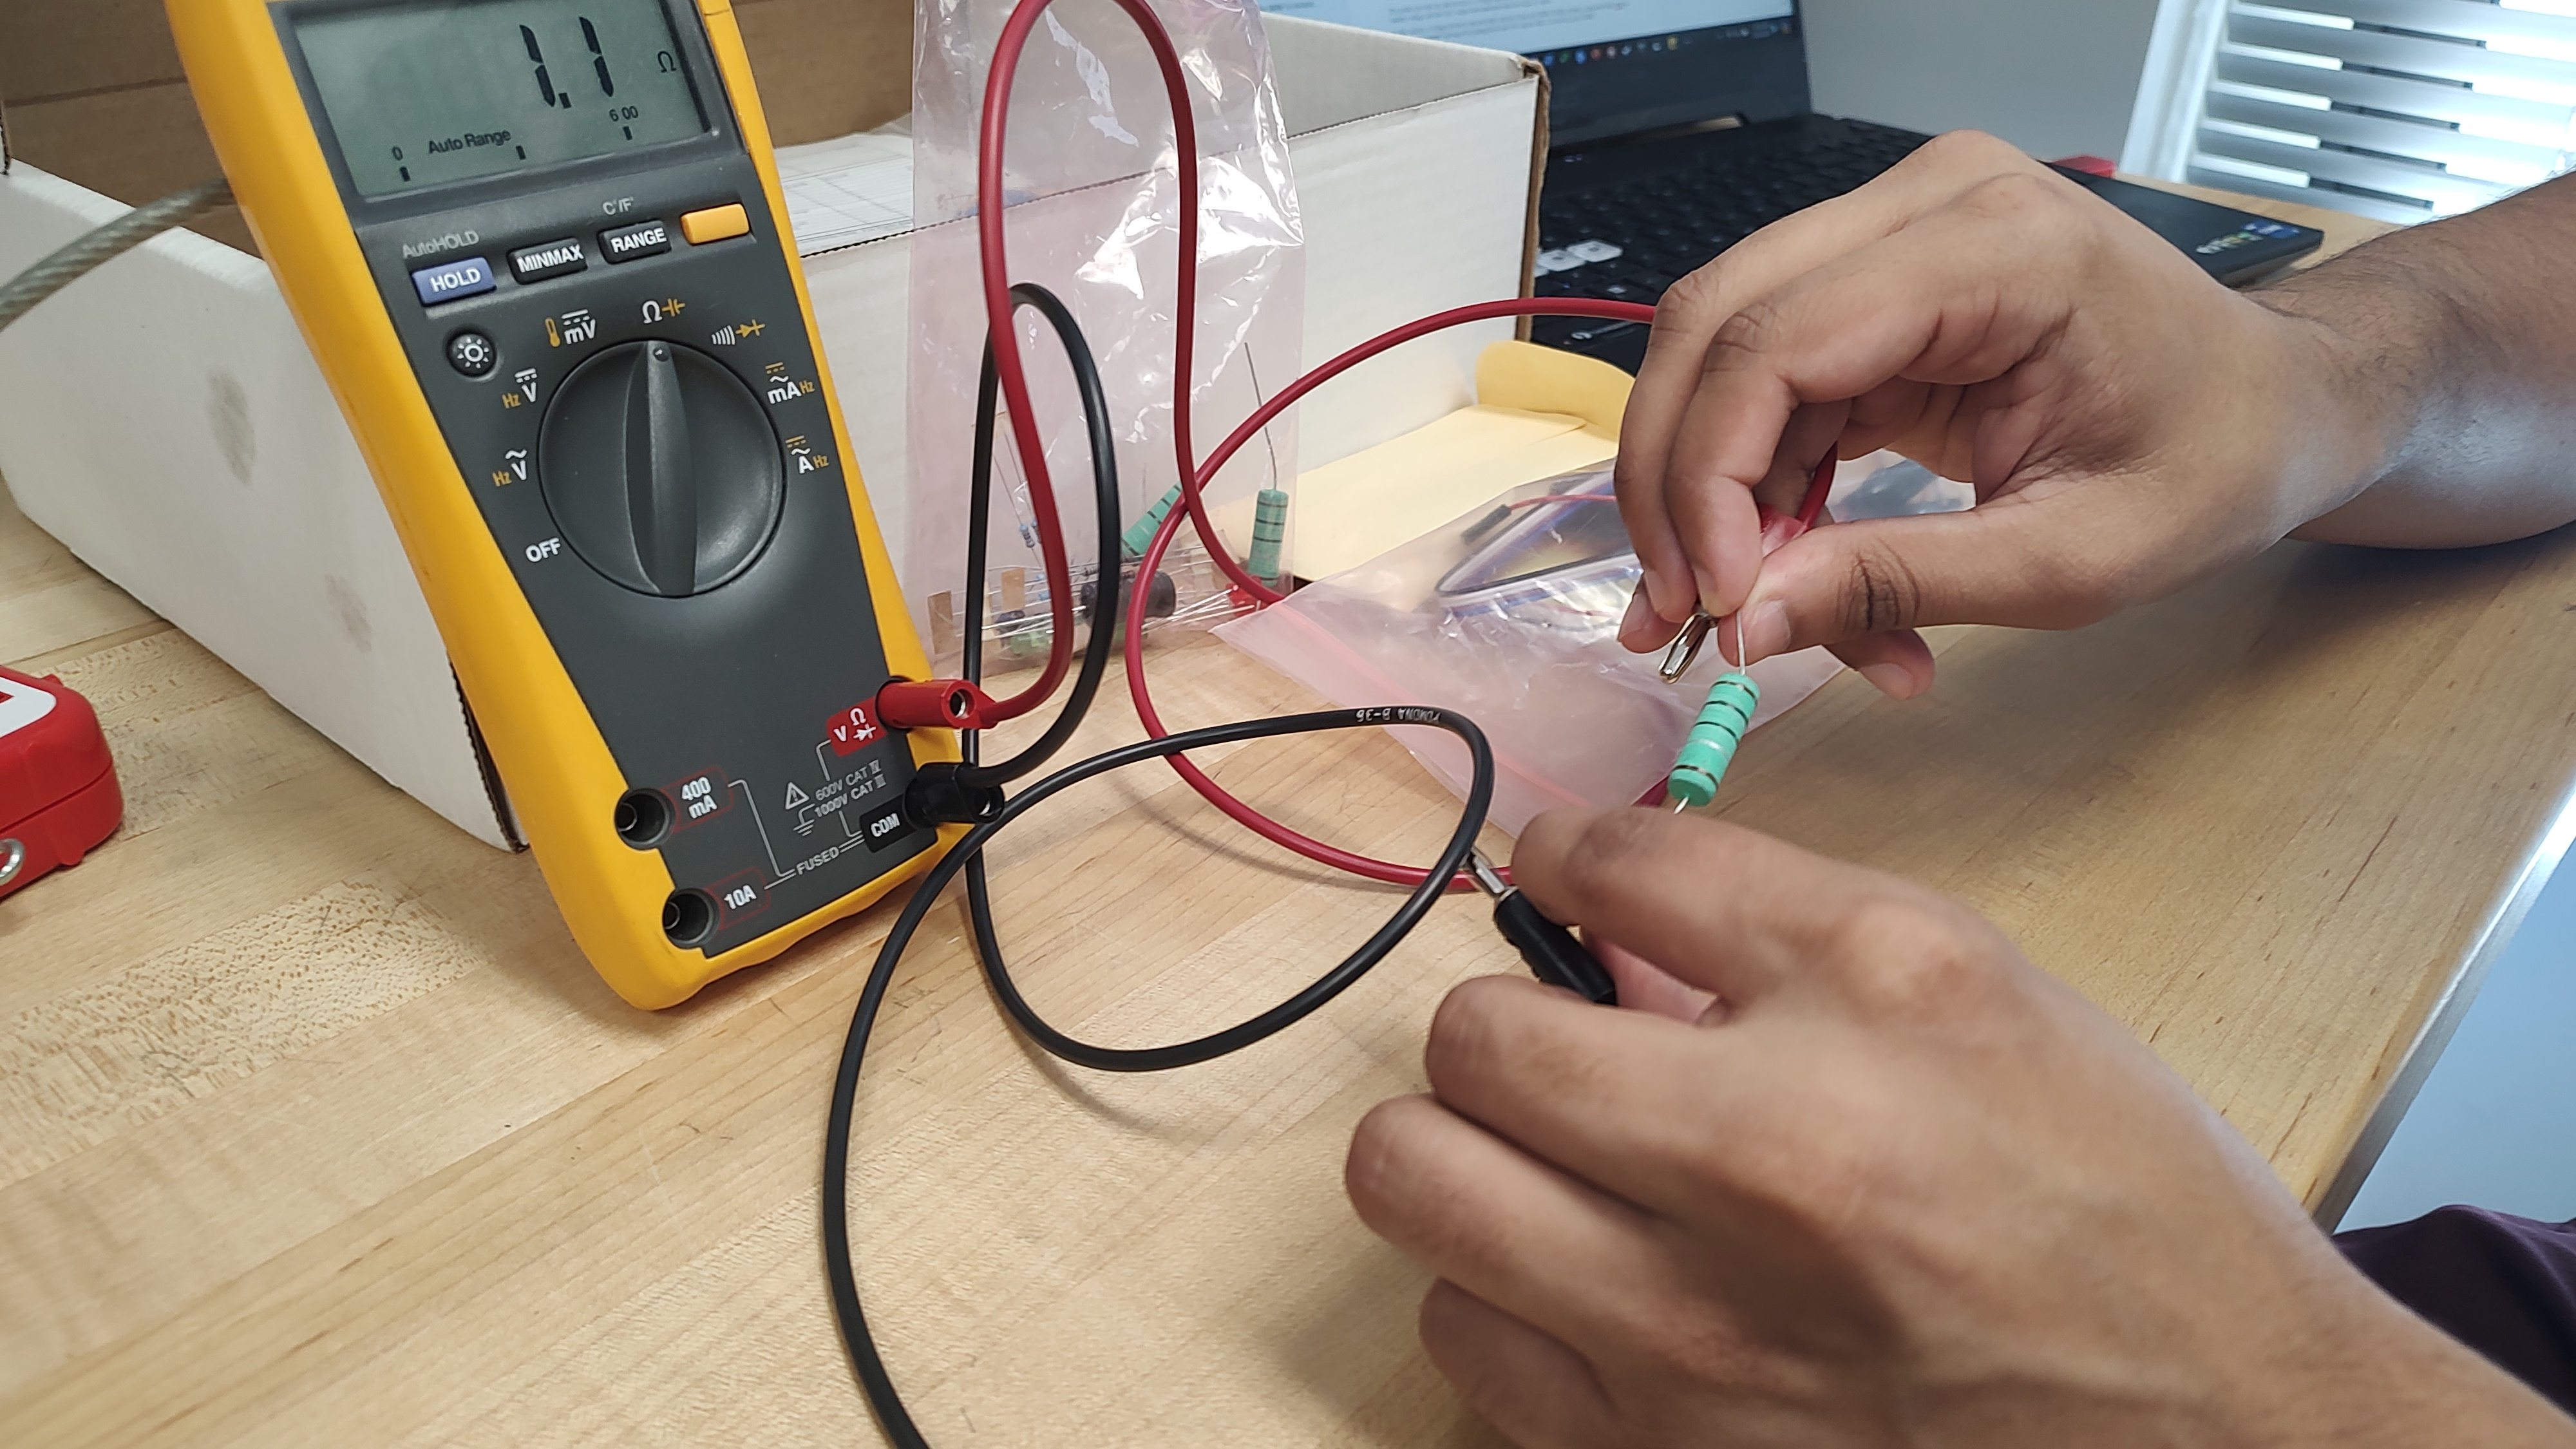
\includegraphics[width=1.0\linewidth]{resources/images/part0_setup}}
            \annotatedFigureBox{0.138,0.3873}{0.348,0.9773}{A}{0.138,0.3873}%bl
            \annotatedFigureBox{0.606,0.424}{0.736,0.5378}{B}{0.606,0.424}%bl
            \annotatedFigureBox{0.586,0.5419}{0.716,0.6907}{C}{0.586,0.5419}%bl
            \annotatedFigureBox{0.54,0.2497}{0.67,0.3983}{D}{0.54,0.2497}%bl
        \end{annotatedFigure}

        \caption{The DMM (A) measures the resistance across a 1 $\Omega$ resistor (B) via banana cables (C) and (D).}
        \label{fig:resistance_setup}
    \end{figure}

    \subsection{Analysis and Conclusion}\label{subsec:resistance_analysis}

    The resistance was measured to be 1.1 $\Omega$.
    The nominal value for the resistance was $1 \pm 1\%~\Omega$.
    The agreement test, from Equation~\ref{eq:agreement_test}, shows that the measured value is within the expected range.
    \begin{e}
        \begin{align*}
            |1.1 - 1| &\le 2 \sqrt{0.1^2 + 0.01^2} \\
            0.1 &\le 2 \sqrt{.0101} \\
            0.1 &\le .201
        \end{align*}
    \end{e}

    This considers the error in the measurement and the error in the expected value.
    The use of a DMM makes human error virtually nonexistent.
    In conclusion, the measured resistance is within the expected range, and the DMM is a reliable tool for measuring resistance.

    \newcounter{section2}
    \renewcommand\thesection{\arabic{section}\Alph{section2}}
    \setcounter{section2}{1}
    \section{Measuring Voltage}\label{sec:voltage}

    \subsection{Methods}\label{subsec:voltage_methods}

    Figure~\ref{fig:current_setup_1a} shows the setup used in this experiment, consisting of a battery and two 10,000 $\Omega$ resistors.
    We measured the voltage at two different parts of the circuit—the initial voltage from the DAC and the voltage after $R_1$.
    We then found the transfer ratio H, found from equation~\ref{eq:transfer_ratio}.

    \begin{figure}[h!]
        \begin{center}
            \begin{circuitikz}[american]
                \draw (0,0) to[battery1=$V_1$, inverted] ++(6,0)
                -- ++(0,-3)
                to[R=$R_1$] ++(-3,0)
                to[R=$R_2$, *-*] ++(-3,0)
                -- ++(0,3);
            \end{circuitikz}
        \end{center}
        \caption {Abstract circuit configuration for measuring current. $R_1$ and $R_2$ are 10,000 $\Omega$ resistors.}
        \label{fig:current_setup_1a}
    \end{figure}

    We used both the IOLab and the DMM to measure the voltage difference.
    We then compared them to see if they agreed.

    \subsection{Analysis}\label{subsec:voltage_analysis}

    When we used the IOLab to measure the voltage difference across $R_1$, we got the graph in figure~\ref{fig:voltage_graph_1a1}.
    \begin{figure}[h!]
        \begin{center}
            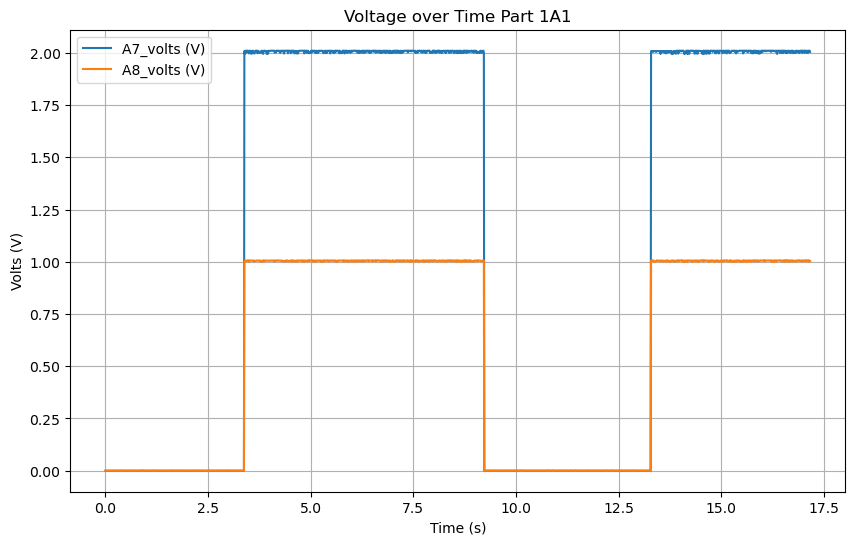
\includegraphics[width=1.0\linewidth]{resources/images/part1a1_voltage_over_time}
        \end{center}
        \caption{Graph of the voltage difference across $R_1$.}
        \label{fig:voltage_graph_1a1}
    \end{figure}

    This graph shows the input (A7) volts and the output (A8) volts.
    When we take the time segment from 4 seconds to 8 seconds, and use equation~\ref{eq:transfer_ratio}, we find the Transfer Ratio $(H): 0.5006 \pm 7.218 * 10^-5$.
    We can use a comparison test, using 1\% as the uncertainty for resistors greater than 1 $\Omega$.
    The error for the transfer ratio is the error for $V$, which is 0.01.
    
    The agreement test, from Equation~\ref{eq:agreement_test}, shows that the measured value is within the expected range.
    \begin{e}
        \begin{align*}
            |0.5 - 0.5006| &\le 2 \sqrt{0.01^2 + 0.00007218^2} \\
            0.0006 &\le 2 \sqrt{.0001} \\
            0.0006 &\le 0.02
        \end{align*}
    \end{e}

    When we used the DMM to measure the voltage difference across $R_1$, we got a value of 1.0 V. We can use a
    comparison test, using 1\% as the uncertainty for resistors greater than 1 $\Omega$.
    We can use the average value from the A8 voltage meter of 1.005 V to compare to the DMM value.
    
    The agreement test, from Equation~\ref{eq:agreement_test}, shows that the DMM and IOLab values agree.
    \begin{e}
        \begin{align*}
            |1.005 - 1| &\le 2 \sqrt{0.01^2 + 0.01^2} \\
            0.0006 &\le 2 \sqrt{.0002} \\
            0.0006 &\le 0.0282
        \end{align*}
    \end{e}

    \subsection{Conclusion}\label{subsec:voltage_conclusion}

    We can see that a voltage divider circuit very evenly divides the voltage between two of the same resistors.
    Also, based on the results obtained from both the IOLab and the DMM measurements of the voltage difference across $R_1$, we can confidently conclude that both instruments yield consistent and reliable readings.
    The comparison tests conducted, along with the agreement test, demonstrate that the values obtained from the two instruments align well with the experiment.
    However, when evaluating voltage divider circuits, potential errors could stem from resistor tolerances, temperature fluctuations, and equipment accuracy.

    \setcounter{section}{0}
    \setcounter{section2}{2}
    \section{Measuring Current}\label{sec:current}

    \subsection{Methods}\label{subsec:current_methods}

    Figure~\ref{fig:current_setup_1b} shows the setup used in this experiment, consisting of a battery, a 10,000 $\Omega$ resistor, and a 1 $\Omega$ resistor.
    We measured the current across $R_2$, which is the 1 $\Omega$ resistor, and compared it to the accepted value of 0.2 mA\@.

    \begin{figure}[h!]
        \begin{center}
            \begin{circuitikz}[american]
                \draw (0,0) to[battery1=$V_1$, inverted] ++(6,0)
                -- ++(0,-3)
                to[R=$R_1$] ++(-3,0)
                to[R=$R_2$, *-*] ++(-3,0)
                -- ++(0,3);
            \end{circuitikz}
        \end{center}
        \caption {Abstract circuit configuration for measuring current. $R_2$ is the 1 $\Omega$ resistor which it is measured across. $R_1$ is a 10,000 $\Omega$ resistor.}
        \label{fig:current_setup_1b}
    \end{figure}

    We used both the IOLab and the DMM to measure the current.

    \subsection{Analysis}\label{subsec:current_analysis}

    When we used the IOLab to measure the current, we got graph in figure~\ref{fig:current_graph_1b1}.
    \begin{figure}[h!]
        \begin{center}
            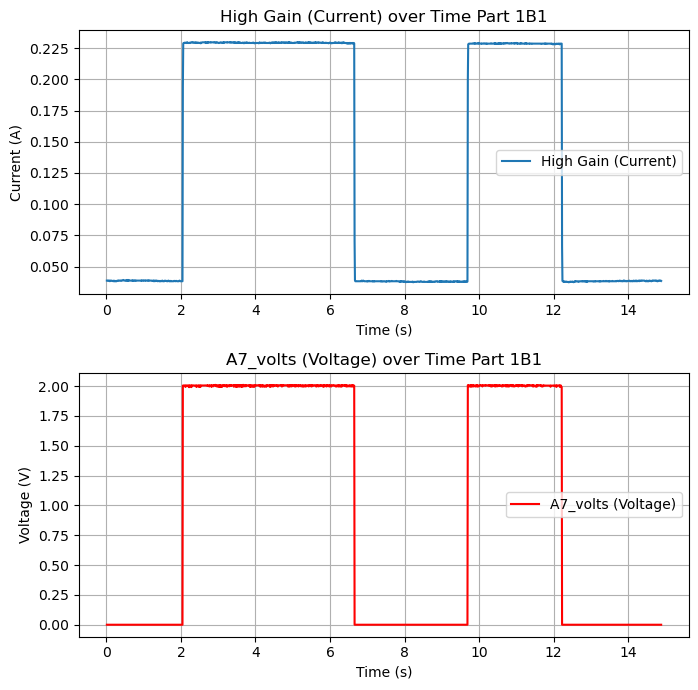
\includegraphics[width=1.0\linewidth]{resources/images/part1b1_voltage_over_time}
        \end{center}
        \caption{Graph of the voltage difference across $R_2$.}
        \label{fig:current_graph_1b1}
    \end{figure}

    This graph shows the input (A7) volts and the current.
    When we take the time segment from 2.5 seconds to 6 seconds, we find the average current to be 0.2294 +- 1.189e-05.
    We can use a comparison test, using 1\% as the uncertainty for resistors greater than 1 ohm.

    The agreement test, from Equation~\ref{eq:agreement_test}, shows that the measured value is not within the expected range.
    \begin{e}
        \begin{align*}
            |0.2294 - 0.2| &\ge 2 \sqrt{0.01^2 + 0.00001189^2} \\
            0.0294 &\ge 2 \sqrt{.0001} \\
            0.0294 &\ge 0.02
        \end{align*}
    \end{e}

    When we used the DMM to measure the current, we got a value of 0.2 mA. This is the same as the accepted value.
    We can see that the IOLab has a higher sensitivity due to it having more decimals as well as being more off from the accepted value, suggesting it picked up unaccounted for error.

    \subsection{Conclusion}\label{subsec:current_conclusion}

    When using the IOLab, our analysis revealed an average current of 0.2294 mA over a specific time interval, with a small uncertainty.
    However, upon conducting comparison and agreement tests, we found that the measured value deviated significantly from the expected range, indicating potential errors.
    Conversely, the DMM measurement yielded a value matching the accepted one.
    The discrepancy between the IOLab and DMM readings highlights differences in sensitivity and potential sources of error.
    The IOLab's higher sensitivity, evident from its more precise measurement, might have led to the detection of unaccounted-for errors, resulting in the observed deviation.
    Conversely, the DMM, with its standard measurement accuracy, provided a value consistent with expectations.
    Possible errors in the current measurement experiment include variations in resistor tolerances, temperature effects on resistance, differences in instrument calibration, potential measurement technique inaccuracies, sampling interval limitations, and human errors in experiment setup or data recording.
    These factors could have contributed to the observed discrepancies between the IOLab and DMM measurements.

    \renewcommand\thesection{\arabic{section}}
    \section{Ohmic and Non-Ohmic Behavior}\label{sec:ohmic}

    \subsection{Methods}\label{subsec:ohmic_methods}

    To verify Ohm's Law, we set up a circuit with a 10,000 $\Omega$ resistor.
    The IOLab was used to provide a voltage to the circuit.
    The DMM was used to measure the voltage across the resistor.
    This can be seen in Figure~\ref{fig:ohmic_setup}.
    The IOLab was set to provide a voltage ranging from 1 V to 3.3 V\@.

    \begin{figure}[h!]
        \begin{annotatedFigure}
        {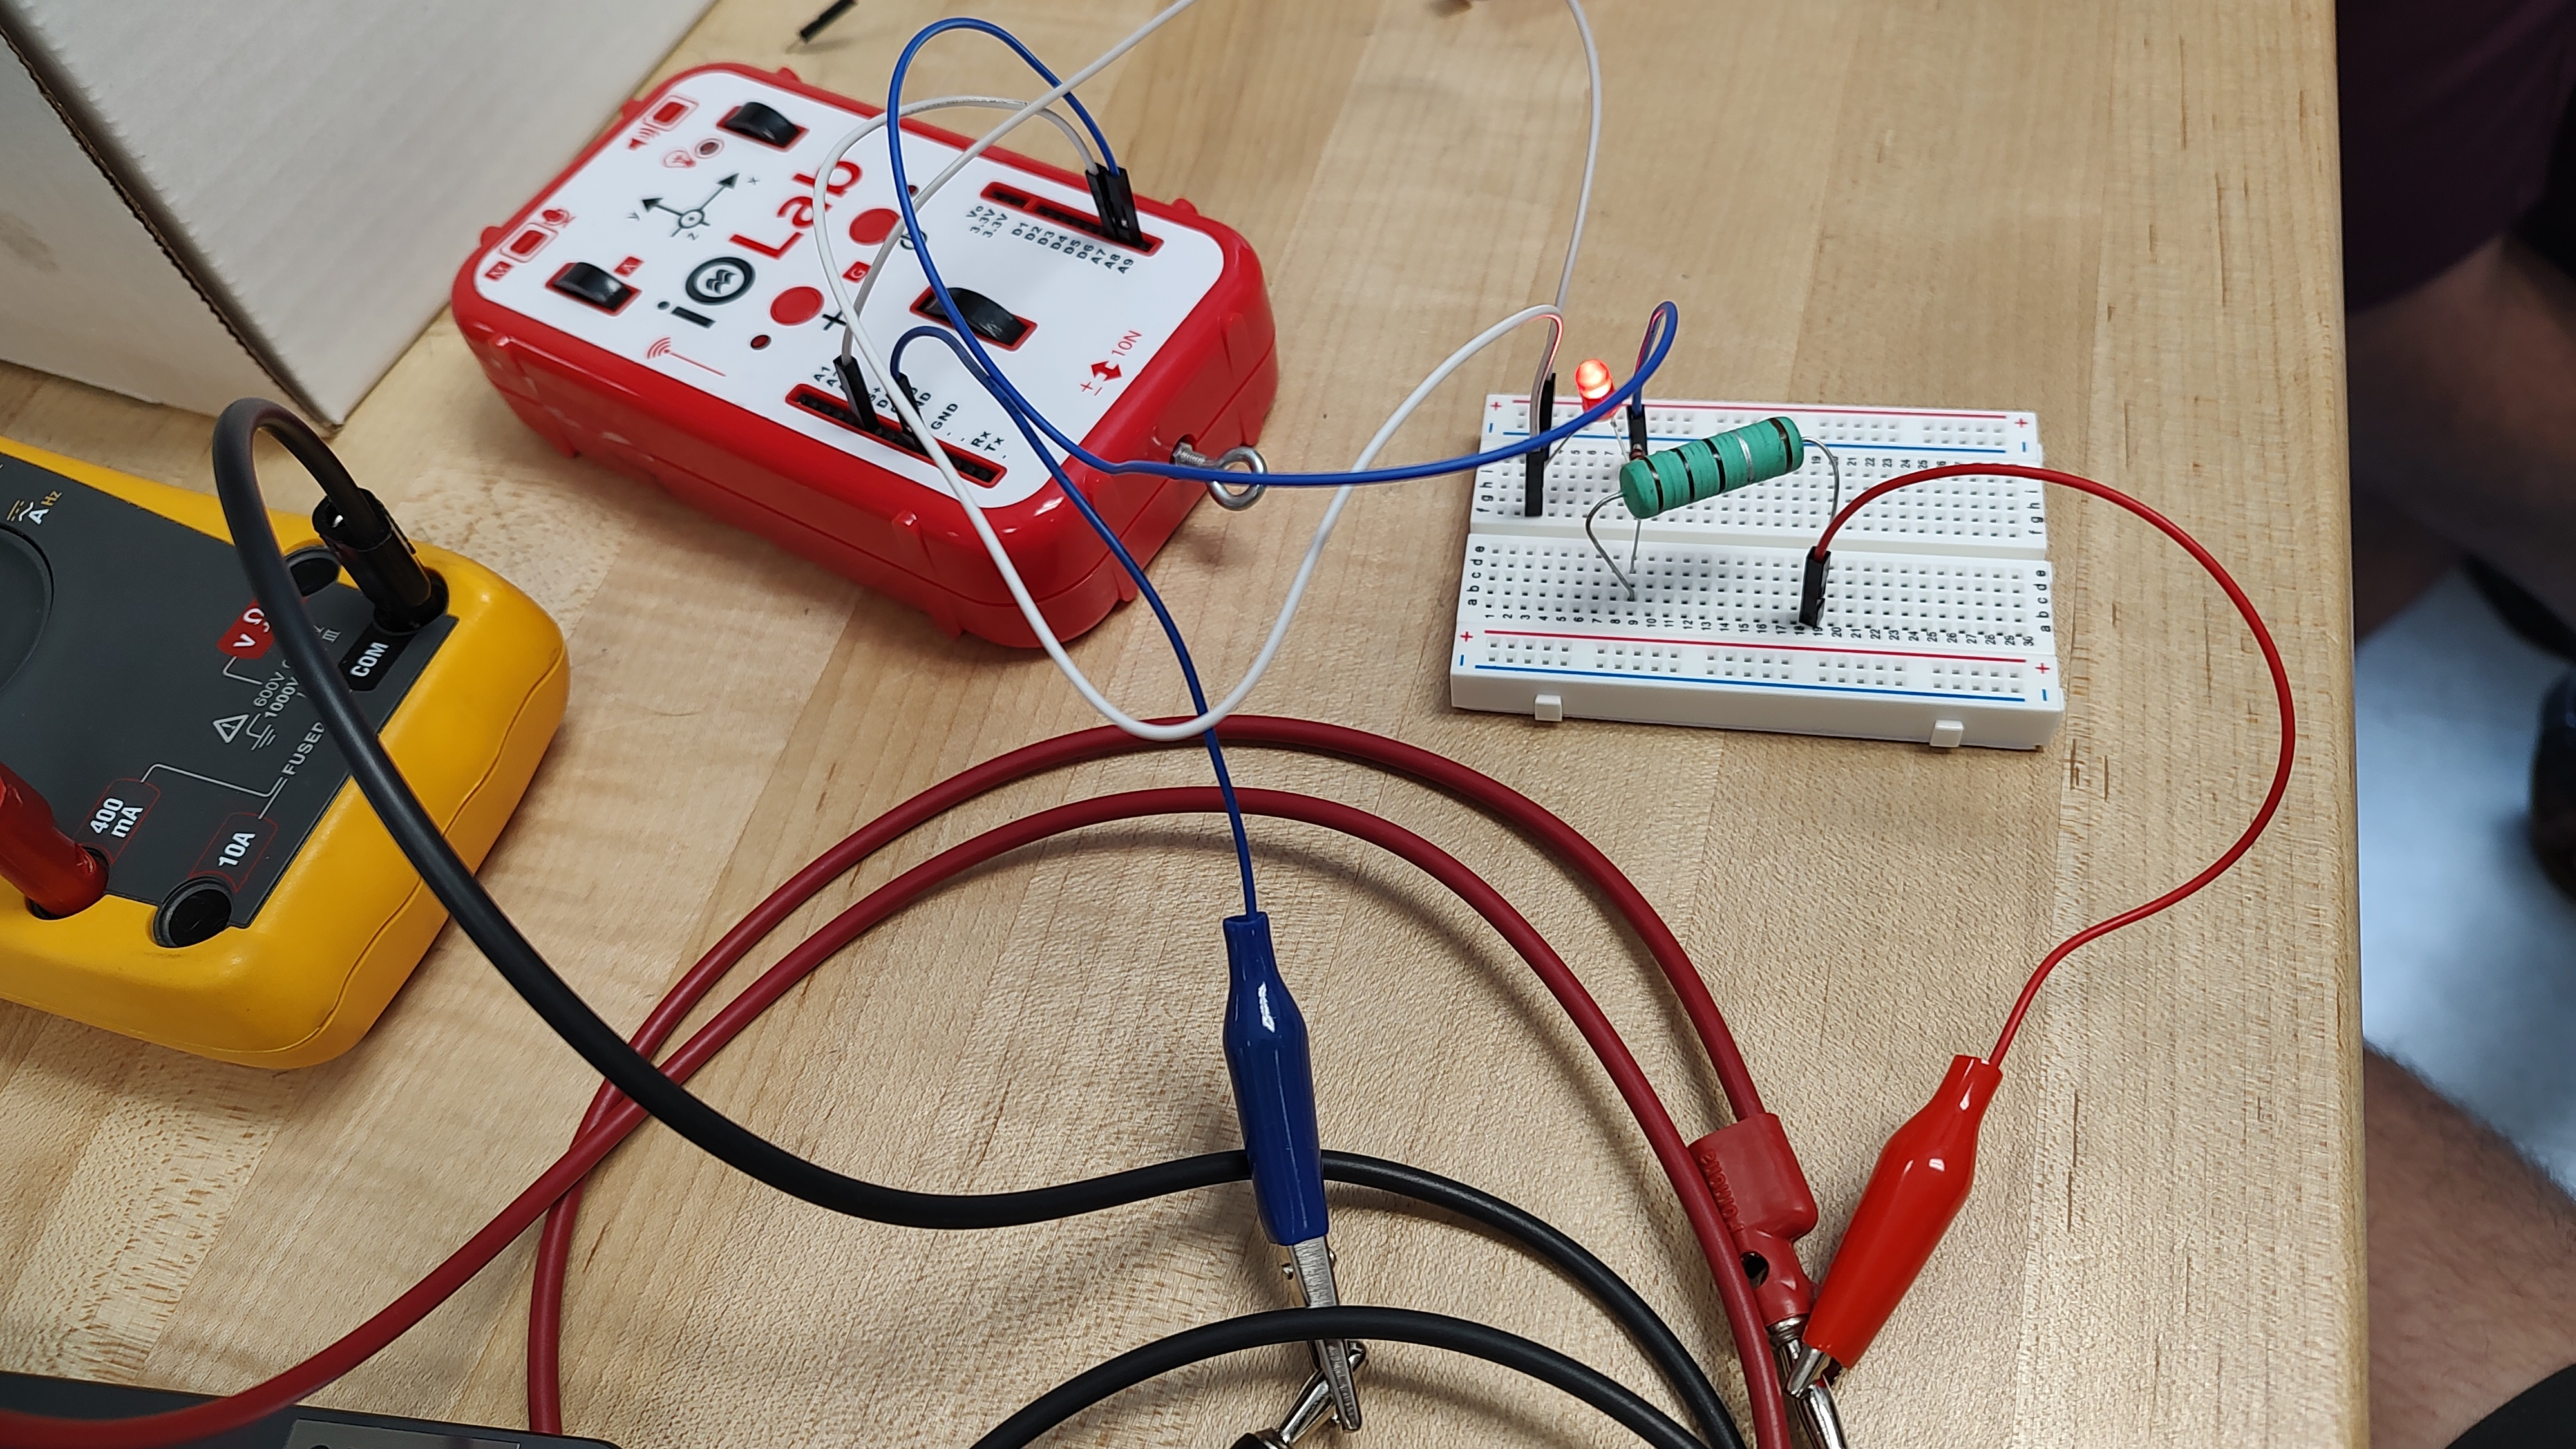
\includegraphics[width=1.0\linewidth]{resources/images/part2_setup}}
            \annotatedFigureBox{0.196,0.6112}{0.483,0.946}{A}{0.196,0.6112}%bl
            \annotatedFigureBox{0.642,0.6217}{0.7352,0.7262}{B}{0.642,0.6217}%bl
            \annotatedFigureBox{0.585,0.6934}{0.639,0.7834}{C}{0.585,0.6934}%bl
            \annotatedFigureBox{0.011,0.3155}{0.177,0.6714}{D}{0.011,0.3155}%bl
        \end{annotatedFigure}
        \caption{The IOLab (A) provides a voltage that runs through the breadboard. On the board a 10 k$\Omega$ resistor (B) is in series. The ground is connected via banana cables that go through the DMM (D).}
        \label{fig:ohmic_setup}
    \end{figure}
    
    First, we measured Ohmic behavior.
    The DMM was set to measure voltage, and the banana cables were connected to the resistor.
    We recorded the voltage across the resistor as the voltage was increased.
    This resulted in the data shown in Figure~\ref{fig:ohmic_data}.


    We measured non-ohmic behavior for two different LEDs, one green and one red.
    The LED was connected in series with a 1 k$\Omega$ resistor.
    We recorded the voltage across the LED as the DAC voltage was increased.
    This resulted in the green LED data shown in Figure~\ref{fig:non_ohmic_data_green} and the red LED data shown in Figure~\ref{fig:non_ohmic_data_red}.

    The residuals for the ohmic behavior can be seen in Figure~\ref{fig:ohmic_residuals}.
    The residuals for the LEDs can be seen in Figure~\ref{fig:non_ohmic_residuals_green} and Figure~\ref{fig:non_ohmic_residuals_red}.
    Each show that the data is random and does not have a pattern, implying that the linear model is a good fit for the data.

    \subsection{Analysis}\label{subsec:ohmic_analysis}

    The data for the ohmic behavior can be seen in Figure~\ref{fig:ohmic_data}.
    When graphed, it shows a linear relationship between voltage and current, as seen in Figure~\ref{fig:ohmic_graph}.
    \begin{figure}[h!]
        \centering
        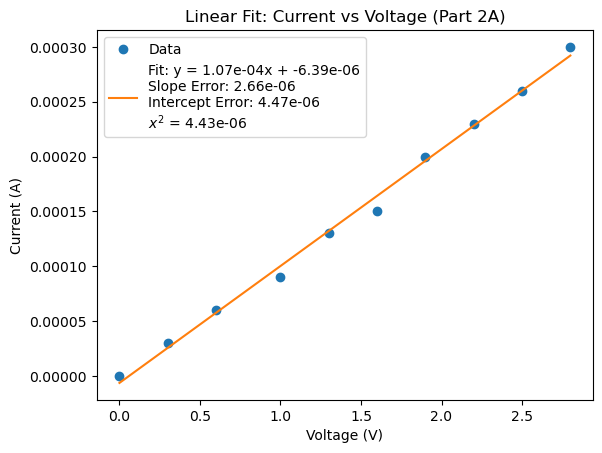
\includegraphics[width=1.0\linewidth]{resources/images/part2a_ohmic_graph}
        \caption{Graph of the ohmic behavior data. \todo{error bars}} % TODO: error bars
        \label{fig:ohmic_graph}
    \end{figure}

    Using equation~\ref{eq:resistance_equation}, we can find the resistance of the resistor.
    \begin{e}
        \begin{align*}
            R &= \frac{V}{I} \\
            R &= \frac{3.3}{0.00032} \\
            R &= 9379.79 \pm 233.97 \Omega
        \end{align*}
    \end{e}
    This ends up differing from the accepted value of 10,000 $\Omega$.
    We can use an agreement test from equation~\ref{eq:agreement_test}, using 1\% as the uncertainty for resistors
    greater than 1 $\Omega$.
    The error for the resistance is the error for $V$, that is 0.01.
    \begin{e}
        \begin{align*}
            |9379.79 - 10000| &\le 2 \sqrt{0.01^2 + 233.97^2} \\
            620.21 &\le 2 \sqrt{54744.0001} \\
            620.21 &\le 466.5
        \end{align*}
    \end{e}
    The agreement test shows that the measured value is not within the expected range.


    The data for the non-ohmic behavior can be seen in Figure~\ref{fig:non_ohmic_data_green} and Figure~\ref{fig:non_ohmic_data_red}.
    When graphed, it shows a linear relationship between voltage and current, as seen in Figure~\ref{fig:non_ohmic_graph}.
    \begin{figure}[h!]
        \centering
        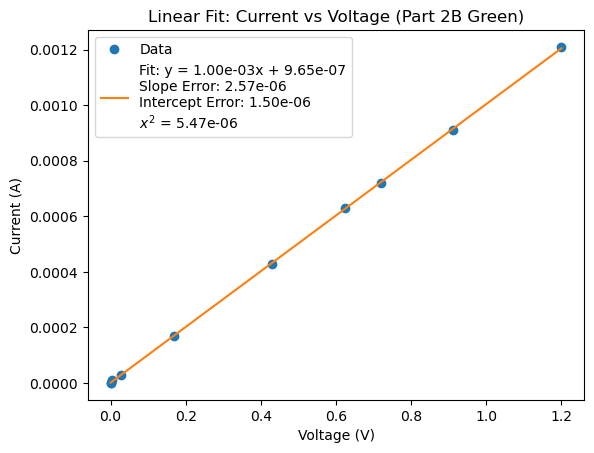
\includegraphics[width=1.0\linewidth]{resources/images/part2_non_ohmic_graph}
        \caption{Graph of the non-ohmic behavior data. \todo{error bars}} % TODO: error bars
        \label{fig:non_ohmic_graph}
    \end{figure}
    The red LED data shows similar relationship between voltage and current, as seen in Figure~\ref{fig:non_ohmic_graph_red}.
    \begin{figure}[h!]
        \centering
        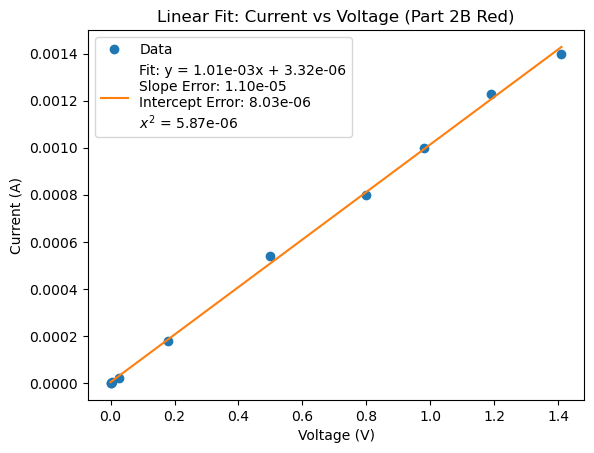
\includegraphics[width=1.0\linewidth]{resources/images/part2_non_ohmic_data_red}
        \caption{Graph of the non-ohmic behavior data for the red LED. \todo{error bars}} % TODO: error bars
        \label{fig:non_ohmic_graph_red}
    \end{figure}

    The non-ohmic behavior is from the LED acting like a wall until a minimum voltage is met, then acting like a wire.
    This is why it makes sense that the data is linear after a certain point.
    Measurements before the minimum voltage were unsuccessful, as the LED was using all the provided voltage, so the current was 0 by equation~\ref{eq:resistance_equation}.

    The resistance can again be found using equation~\ref{eq:resistance_equation}.
    This calculation results in a resistance of $996.50 \pm 2.56 \Omega$ for the green LED and $989.35 \pm 10.81 \Omega$ for the red LED\@.
    \begin{e}
        \begin{align*}
            R &= \frac{V}{I} \\
            R_{green} &= 996.50 \pm2.56 \Omega \\
            R_{red} &= 989.35 \pm10.81 \Omega
        \end{align*}
    \end{e}

    These results mean that the green LED and red LED both acted like wires once the minimum voltage was met, so it
    allowed us to properly measure resistance.
    We can use an agreement test from equation~\ref{eq:agreement_test}, using 1\% as the uncertainty for resistors:
    \begin{e}
        \begin{align*}
            |996.50 - 1000| &\le 2 \sqrt{0.01^2 + 2.56^2} \\
            3.5 &\le 2 \sqrt{6.5156} \\
            3.5 &\le 5.1 \\
            |989.35 - 1000| &\le 2 \sqrt{0.01^2 + 10.81^2} \\
            10.65 &\le 2 \sqrt{116.6561} \\
            10.65 &\le 21.6
        \end{align*}
    \end{e}
    The agreement test shows that the measured value is within the expected range.

    The chi-squared test for the green LED is 0.0001, and for the red LED is 0.0002.
    This means that the green LED is a better fit to the linear model than the red LED\@.
    However, both values are very close to 0 and too small, meaning that neither linear model is a good fit for the LEDs.
    This is likely because the data did not vary enough to provide a larger chi-squared value.

    
    \subsection{Conclusion}\label{subsec:ohmic_conclusion}

    The data for the ohmic behavior shows a linear relationship between voltage and current, as seen in Figure~\ref{fig:ohmic_graph}.
    However, the resistance of the resistor was found to be $9379.79 \pm 233.97 \Omega$, which is slightly out of range of the accepted value.
    The data for the non-ohmic behavior shows a non-linear relationship between voltage and current, as seen in Figure~\ref{fig:non_ohmic_graph} and Figure~\ref{fig:non_ohmic_graph_red}.
    This linear relationship only begins after a minimum voltage is met, which is likely due to the LED acting like a wire once the minimum voltage is met.
    Beforehand, the LED acts like a wall.

    The red LED has a higher resistance than the green LED, which is likely due to the red LED having a higher
    voltage drop than the green LED\@.
    This is because it is a larger wavelength, and thus has a larger energy gap, which requires more energy to pass through.
    After the minimum voltage is met, the LED acts like a wire, so the resistance is the same as the other resistor in series with it.


    \section{Kirchhoff's Laws}\label{sec:kirchoff}

    \subsection{Methods}\label{subsec:kirchoff_methods}

    \begin{figure}[h!]
        \begin{center}
            \begin{circuitikz}[american]
                \draw (0,0) to[battery1=$V_1$] ++(0,3)
                to[R=$R_1$] ++(3,0) coordinate(P1)
                to[R=$R_3$, -*] ++(0,-3)
                node[above right] {$A$}
                -- (0,0);
                \draw (P1) to[R=$R_2$] ++(3,0)
                to[battery1, l=$V_2$] ++(0,-3) -- ++(-3,0);
            \end{circuitikz}
        \end{center}
        \caption {Abstract circuit configuration for Kirchhoff's Laws experiment.}
        \label{fig:kirchoff_setup}
    \end{figure}

    For this experiment, we set up a circuit with three resistors, $R_1$, $R_2$, and $R_3$, measuring 4.7k, 10k, and 4.7k $\Omega$, respectively.
    The goal was to measure the current before and after Junction $A$.
    To measure the current, we placed 1 $\Omega$ resistors before and after the junction.
    This can be seen in Figure~\ref{fig:kirchoff_setup}.
    We then used the DMM to measure the voltage across the resistors.
    The 1 $\Omega$ resistors added a negligible amount of resistance to the circuit, allowing them to act as ammeters.

    \subsection{Analysis}\label{subsec:kirchoff_analysis}

    Given figure~\ref{fig:kirchoff_setup}, we can use Kirchhoff's Laws to analyze the expected currents in the circuit.
    Taking $I_1$ as the initial current from the DAC ($V_1$) flowing into $R_1$, $I_2$ as the current after the batterie ($V_2$) flowing into $R_2$, and $I_3$ as the current after the resistor $R_3$, we can use the following equations:
    \begin{align*}
        Loop~1: V_1 - I_1 R_1 - I_2 R_2 &= 0 \\
        Loop~2: V_2 - I_2 R_2 - I_3 R_3 &= 0 \\
        Junction~A: I_3 - I_2 - I_1 &= 0
    \end{align*}
    These equations give:
    \begin{align*}
        I_1 &= \frac{V_1(R_2 + R_3) - V_2 R_3}{R_1 R_2 + R_2 R_3 + R_1 R_3} \\
        I_2 &= \frac{V_2(R_1 + R_3) - V_1 R_3}{R_1 R_2 + R_2 R_3 + R_1 R_3} \\
        I_3 &= \frac{V_1 R_2 + V_2 R_1}{R_1 R_2 + R_2 R_3 + R_1 R_3}
    \end{align*}
    For this experiment, we used:
    \begin{align*}
        V_1 &= 3.3 \pm 0.1 \text{ V} \\
        V_2 &= 4.5 \pm 0.1 \text{ V} \\
        R_1 &= 4.7k \pm 0.1k \text{ $\Omega$} \\
        R_2 &= 10k \pm 0.1k \text{ $\Omega$} \\
        R_1 &= 4.7k \pm 0.1k \text{ $\Omega$}
    \end{align*}
    which results in expected values for the currents of:
%    ['I1: 0.236 mA', 'I2: 0.231 mA', 'I3: 0.466 mA']
    \begin{align*}
        I_{1exp} &= 0.236 \pm 0.01 \text{mA} \\
        I_{2exp} &= 0.231 \pm 0.01 \text{mA} \\
        I_{3exp} &= 0.466 \pm 0.01 \text{mA}
    \end{align*}

    With the DMM, we measured the currents to be:
    \begin{align*}
        I_{1mea} &= 0.168 \pm 0.001 \text{mA} \\
        I_{2mea} &= 0.156 \pm 0.001 \text{mA} \\
        I_{3mea} &= 0.504 \pm 0.001 \text{mA}
    \end{align*}

    The agreement test, from Equation~\ref{eq:agreement_test}, shows that the measured values are not within the expected range.
    \begin{e}
        \begin{align*}
            |0.504 - 0.466| &\ge 2 \sqrt{0.001^2 - 0.01^2} \\
            0.038 &\ge 2 \sqrt{.0001} \\
            0.038 &\ge 0.0201
        \end{align*}
    \end{e}

    We also found that our data did not obey Kirchhoff's Junction rule, as we can clearly see that $I_1$ + $I_2$ does not equal $I_3$.
    This means our data was off significantly, and we should not expect it to be within an acceptable range.

    \subsection{Conclusion}\label{subsec:kirchoff_conclusion}

    Based on the analysis conducted using Kirchhoff's Laws and the experimental measurements, it's evident that there are discrepancies between the expected values and the measured values of currents in the circuit. The measured currents do not align with the values predicted by Kirchhoff's Laws, indicating potential errors in the experimental setup or measurements.

    The observed disagreement between the expected and measured currents, along with the violation of Kirchhoff's Junction rule (I1 + I2 ≠ I3), suggests that there are systematic errors or inaccuracies in the experimental setup, measurement instruments, or data collection process.

    It can be concluded that further investigation and troubleshooting are required to identify and rectify the sources of error in the experiment. This may involve rechecking the circuit connections, calibrating measurement instruments, ensuring proper placement and functioning of resistors acting as ammeters, and considering environmental factors that could influence the measurements. Additionally, repeating the experiment with enhanced precision and control measures may be necessary to obtain reliable and accurate results consistent with Kirchhoff's Laws.

    \section{Conclusion}\label{sec:conclusion}

    This laboratory experiment aimed to explore fundamental electrical measurements and circuit analysis techniques using Digital Multimeter's (DMMs) and the IOLab device.
    We seek to validate theoretical concepts through practical experimentation, focusing on resistance measurement, voltage division, current measurement, and application of Kirchhoff's laws.

    In part 0, we measured the resistance of a resistor and performed an agreement test with the nominal value obtained from the color code.
    The DMM provided accurate resistance measurements, offering a reliable tool for such tasks.

    For part 1, experimenting with a voltage divider circuit using both the IOLab and DMM, we verified the transfer ratio and compared experimental values with theoretical ones.
    The IOLab and DMM measurements exhibited good agreement for voltage, demonstrating their efficacy in voltage measurements.
    However, they differed when measuring current.

    In Experiment 2, we investigated Ohm's law using resistors and analyzed the linear relationship between voltage and current.
    However, our measurements were off and couldn't verify the correct measured resistance.
    Experiment 2B explored non-Ohmic behavior using LEDs, highlighting deviations from Ohm's law due to semiconductor properties.
    Our data suggested that the LEDs were not ohmic, as they first acted like walls then acted like wires.

    Finally, in Part 3, we applied Kirchhoff's laws to analyze a complex circuit setup.
    By comparing predicted and measured currents and voltages, we found our measurements were off, meaning we could not verify Kirchhoff's junction rule.

    Through precise resistance measurements with the DMM, analysis of voltage division using both the IOLab and DMM, comparison of current measurement techniques and application of Kirchhoff's laws in circuit analysis, this experiment provided practice using electrical circuits and theory.
    The exploration enhanced our understanding of electrical measurements and equipped us with essential skills for future endeavors in electrical engineering.

    \appendix
    \section{Data}\label{sec:data}

    \begin{figure}[h!]
        \centering
        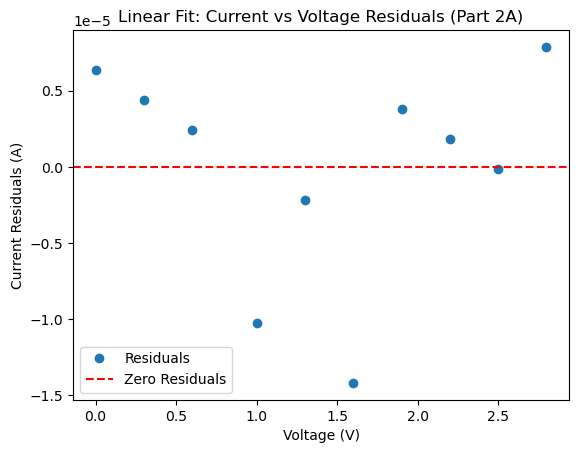
\includegraphics[width=1.0\linewidth]{resources/images/2a_residuals}
        \caption{Residuals for the ohmic behavior data.}
        \label{fig:ohmic_residuals}
    \end{figure}

    \begin{figure}[h!]
        \centering
        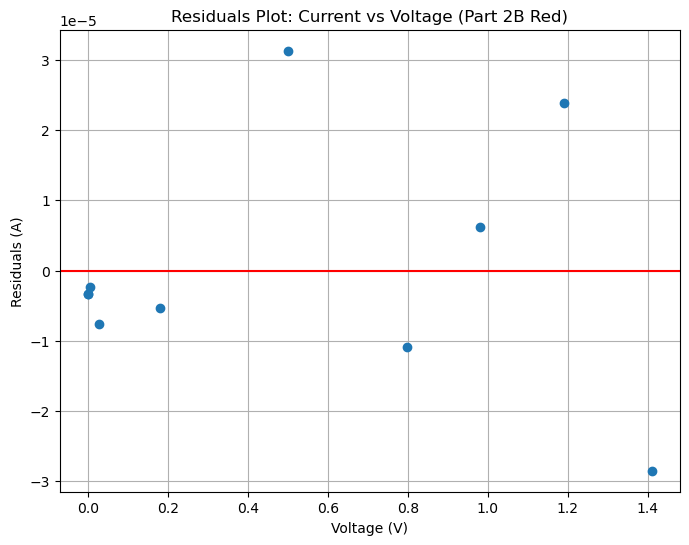
\includegraphics[width=1.0\linewidth]{resources/images/2b2_residuals}
        \caption{Residuals for the green LED behavior data.}
        \label{fig:non_ohmic_residuals_green}
    \end{figure}

    \begin{figure}[h!]
        \centering
        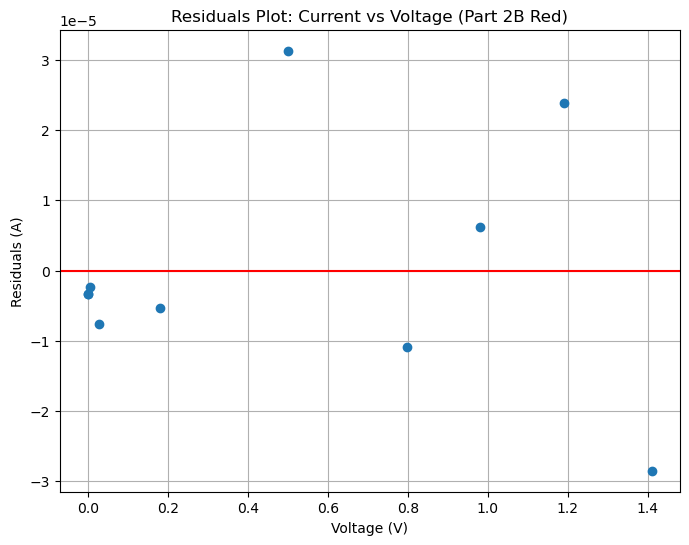
\includegraphics[width=1.0\linewidth]{resources/images/2b3_residuals}
        \caption{Residuals for the non-ohmic behavior data for the red LED.}
        \label{fig:non_ohmic_residuals_red}
    \end{figure}

    \begin{figure}[h!]
        \centering
        \begin{tabular}{|c|c|}
            \hline
            \text{Volts (V)} & \text{Amps (A)} \\
            \hline
            0 & 0 \\
            0.3 & 0.00003 \\
            0.6 & 0.00006 \\
            1.0 & 0.00009 \\
            1.3 & 0.00013 \\
            1.6 & 0.00015 \\
            1.9 & 0.00020 \\
            2.2 & 0.00023 \\
            2.5 & 0.00026 \\
            2.8 & 0.00030 \\
            3.1 & 0.00032 \\
            \hline
        \end{tabular}
        \caption{Voltage and current data for the ohmic experiment.}
        \label{fig:ohmic_data}
    \end{figure}

    \begin{figure}[h!]
        \centering
        \begin{tabular}{|c|c|c|}
            \hline
            \text{A7 (Input) Voltage (V)} & \text{A8 (After LED) Voltage (V)} & \text{Current (A)} \\
            \hline
            1.0 & 0 & 0 \\
            1.3 & 0 & 0 \\
            1.6 & 0.005 & 0.00001 \\
            1.7 & 0.027 & 0.00003 \\
            1.9 & 0.17 & 0.00017 \\
            2.2 & 0.43 & 0.00043 \\
            2.4 & 0.624 & 0.00063 \\
            2.5 & 0.72 & 0.00072 \\
            2.8 & 0.91 & 0.00091 \\
            3.1 & 1.20 & 0.00121 \\
            3.3 & 1.37 & 0.00138 \\
            \hline
        \end{tabular}
        \caption{Voltage and current data for the green LED experiment.}
        \label{fig:non_ohmic_data_green}
    \end{figure}

    \begin{figure}[h!]
        \centering
        \begin{tabular}{|c|c|c|}
            \hline
            \text{A7 (Input) Voltage (V)} & \text{A8 (After LED) Voltage (V)} & \text{Current (A)} \\
            \hline
            0.8 & 0 & 0 \\
            1.0 & 0 & 0 \\
            1.3 & 0.004 & 0.000005 \\
            1.6 & 0.027 & 0.000023 \\
            1.8 & 0.18 & 0.00018 \\
            2.1 & 0.50 & 0.00054 \\
            2.3 & 0.799 & 0.0008 \\
            2.5 & 0.98 & 0.001 \\
            2.8 & 1.19 & 0.00123 \\
            3.1 & 1.41 & 0.00140 \\
            3.3 & 1.67 & 0.00165 \\
            \hline
        \end{tabular}
        \caption{Voltage and current data for the red LED experiment.}
        \label{fig:non_ohmic_data_red}
    \end{figure}

    \section{References}\label{sec:references}

    Lab Manual

\end{document}